\chapter{Resultados}

Na tabela \ref{estadoAtual} pode ser visualizado as Histórias de Usuário, a pontuação e o estado (a fazer, em progresso ou feito) de cada História. Foram implementados 12 pontos do total de 48 pontos estimados. Sendo assim, já foi implementado 25\% dos pontos da ferramenta InvestMVC.

\begin{table}[H]
\caption{Estado atual da ferramenta InvestMVC}
\begin{center}
    \begin{tabular}{ | c | c | c |}
    \hline
    \textbf{Histórias de Usuário} & \textbf{Pontuação} & \textbf{Estado} \\ \hline

US1 - Agente Correlação Linear & 3 & Em progresso\\ \hline
US2 - Agente Fibonacci & 3 & A fazer \\ \hline
US3 - Agente Mínimos Quadrados & 3 & A fazer\\ \hline
US4 -  Agente Tendência & 2 & Em progresso\\ \hline
US5 - Agente Gestor/Consultor & 2& Em progresso\\ \hline
US6 - Criar conta de usuário & 2 & Feito\\ \hline
US7 - Acompanhar retorno financeiro & 5 & A fazer\\ \hline
US8 - Criar Experts & 2 & Feito\\ \hline
US9 - Editar Experts & 2 & Feito\\ \hline
US10 - Excluir Experts & 2 & Feito\\ \hline
US11 - Ativar Expert & 1 & A fazer\\ \hline
US12 - Desativar Expert & 2 & A fazer \\ \hline
US13 - Método Correlação Linear em linguagem C & 2 & Feito\\ \hline
US14 - Método Fibonacci em linguagem C & 2 & Feito\\ \hline
US15 - Método Mínimos Quadrados em linguagem C & 2 & Feito\\ \hline
US16 - Método Correlação Linear em linguagem Haskell & 2 & Em progresso\\ \hline
US17 - Método Fibonacci em linguagem Haskell & 2 & Em progresso\\ \hline
US18 - Método Mínimos Quadrados em linguagem Haskell & 2 & Em progresso\\ \hline
US19 - Inserir na Base de Conhecimento & 2 & A fazer\\ \hline
US20 - Retirar na Base de Conhecimento & 2 & A fazer\\ \hline
US21 - Calcular Critério de Entrada & 3 & A fazer\\ \hline
US22 - Realizar Operação no MetaTrader& 1 & Feito\\ \hline
\end{tabular}
\end{center}
\label{estadoAtual}
\end{table}

\section{Resultados do Componente Orientado a Objetos}
No apêndice C - Componente OO, encontra-se o código fonte das Classes Modelo Expert e User, implementadas em liguagem Groovy. No apêndice C também encontra-se as telas da ferramenta InvestMVC. Um exemplo de tela da ferramenta InvestMVC é exposta na figura \ref{telaInicial}

\begin{figure}[H]
\centering
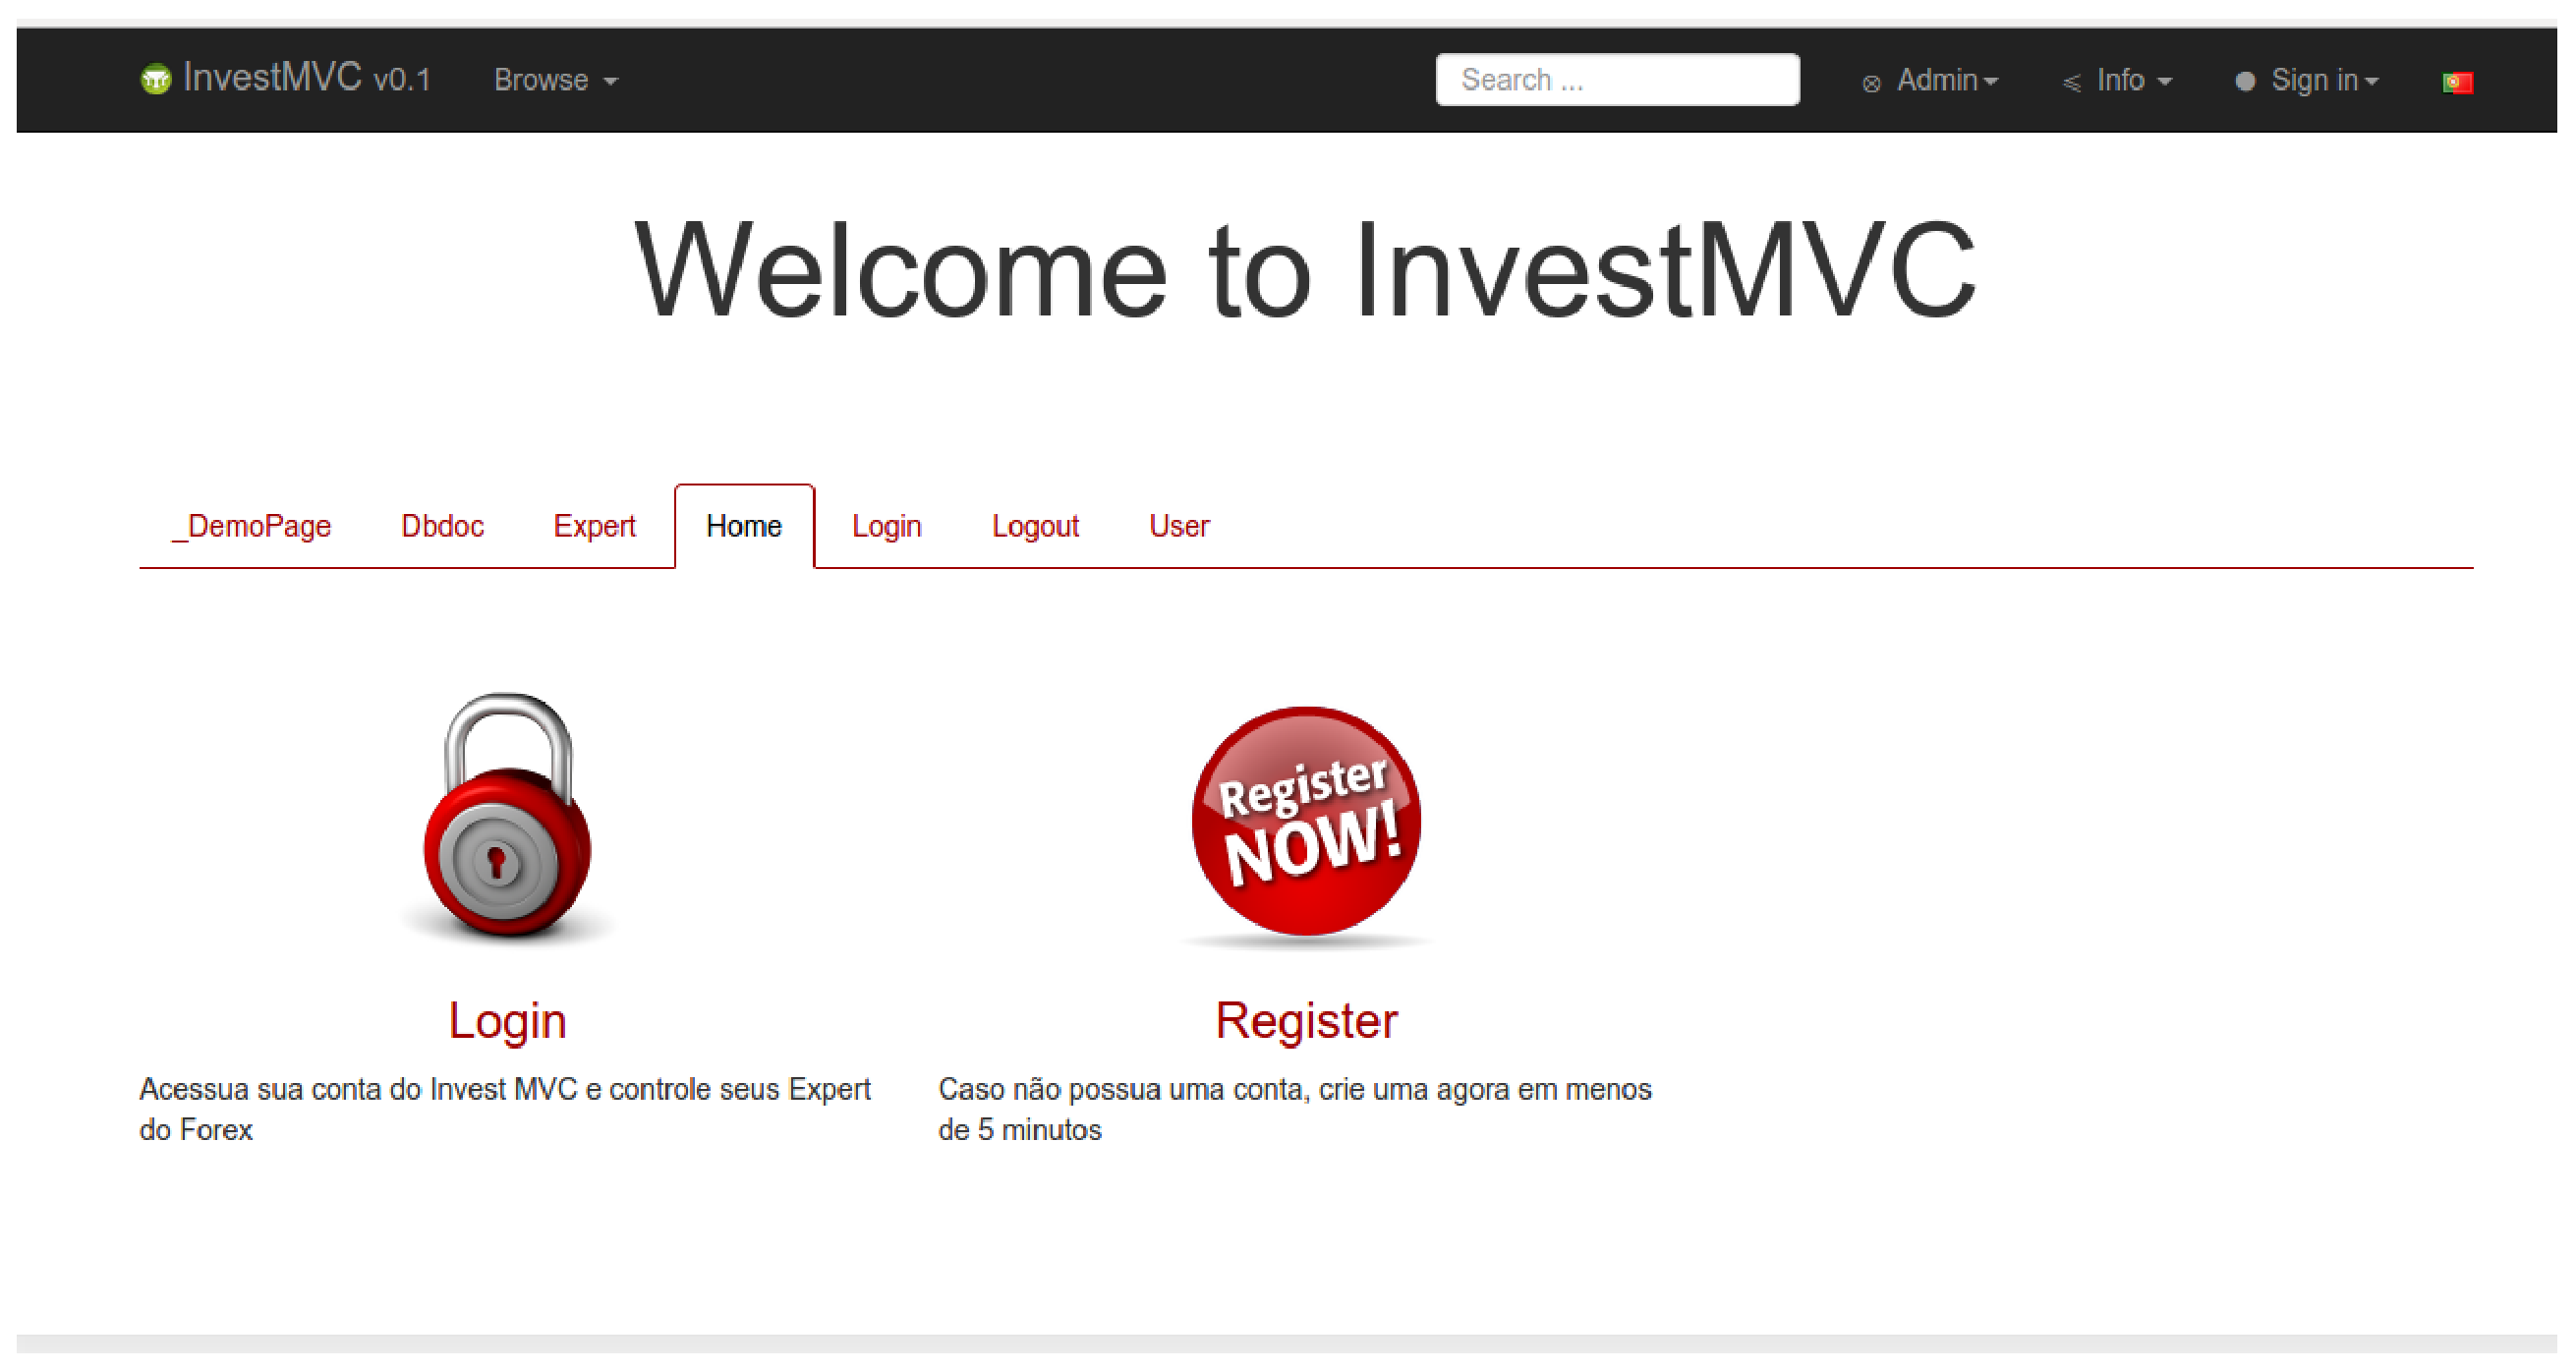
\includegraphics[width=0.9\textwidth]{figuras/telaInicial}
\caption{Tela Inicial da ferramenta InvestMVC}
\label{telaInicial}
\end{figure}

\section{Resultados do Componente Funcional}
No apêndice D - Componente Funcional, encontra-se o código fonte do Método de Correlação Linear em linguagem Haskell (US16) juntamente com seu teste unitário.

Na figura \ref{testeHaskel} é possível perceber que os testes unitários foram executados se falhas.
 
\begin{figure}[H]
\centering
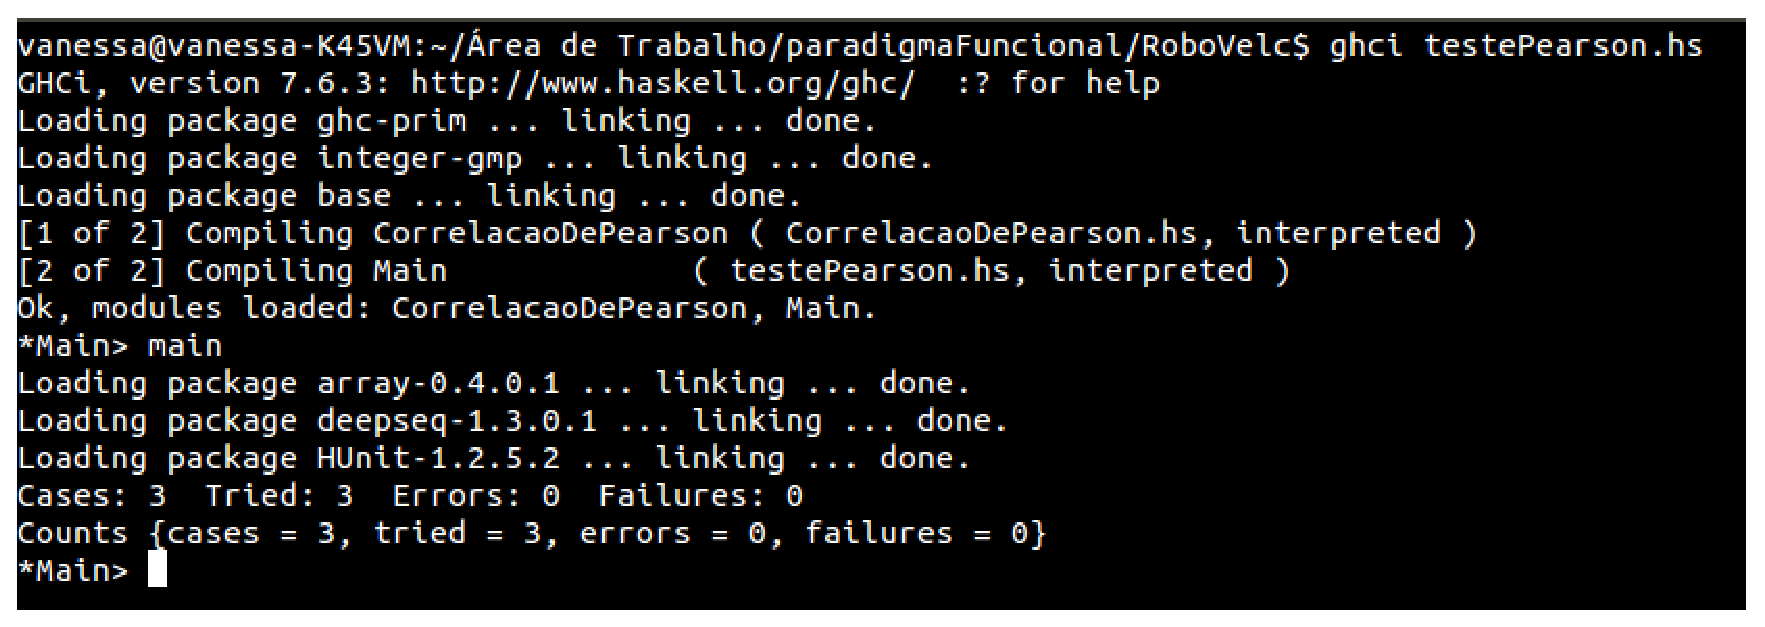
\includegraphics[width=0.9\textwidth]{figuras/testeHaskel}
\caption{Suíte de Teste do Componente Funcional InvestMVC}
\label{testeHaskel}
\end{figure}

\section{Resultados do Componente Estruturado}

Encontra-se no apêndice E,  o código fonte das Histórias de Usuário 13 (Método de Correlação Linear em linguagem C), 14 (Método de Fibonacci em linguagem C) e 15 (Método de Mínimos Quadrados em linguagem C). No mesmo apêndice segue o teste unitário de cada História de Usuário.

Na figura \ref{coberturaEstrturado} é possível ver o resultado da suite de teste do Componente Estruturado. A cobertura de código encontra-se em 100\%.

\begin{figure}[H]
\centering
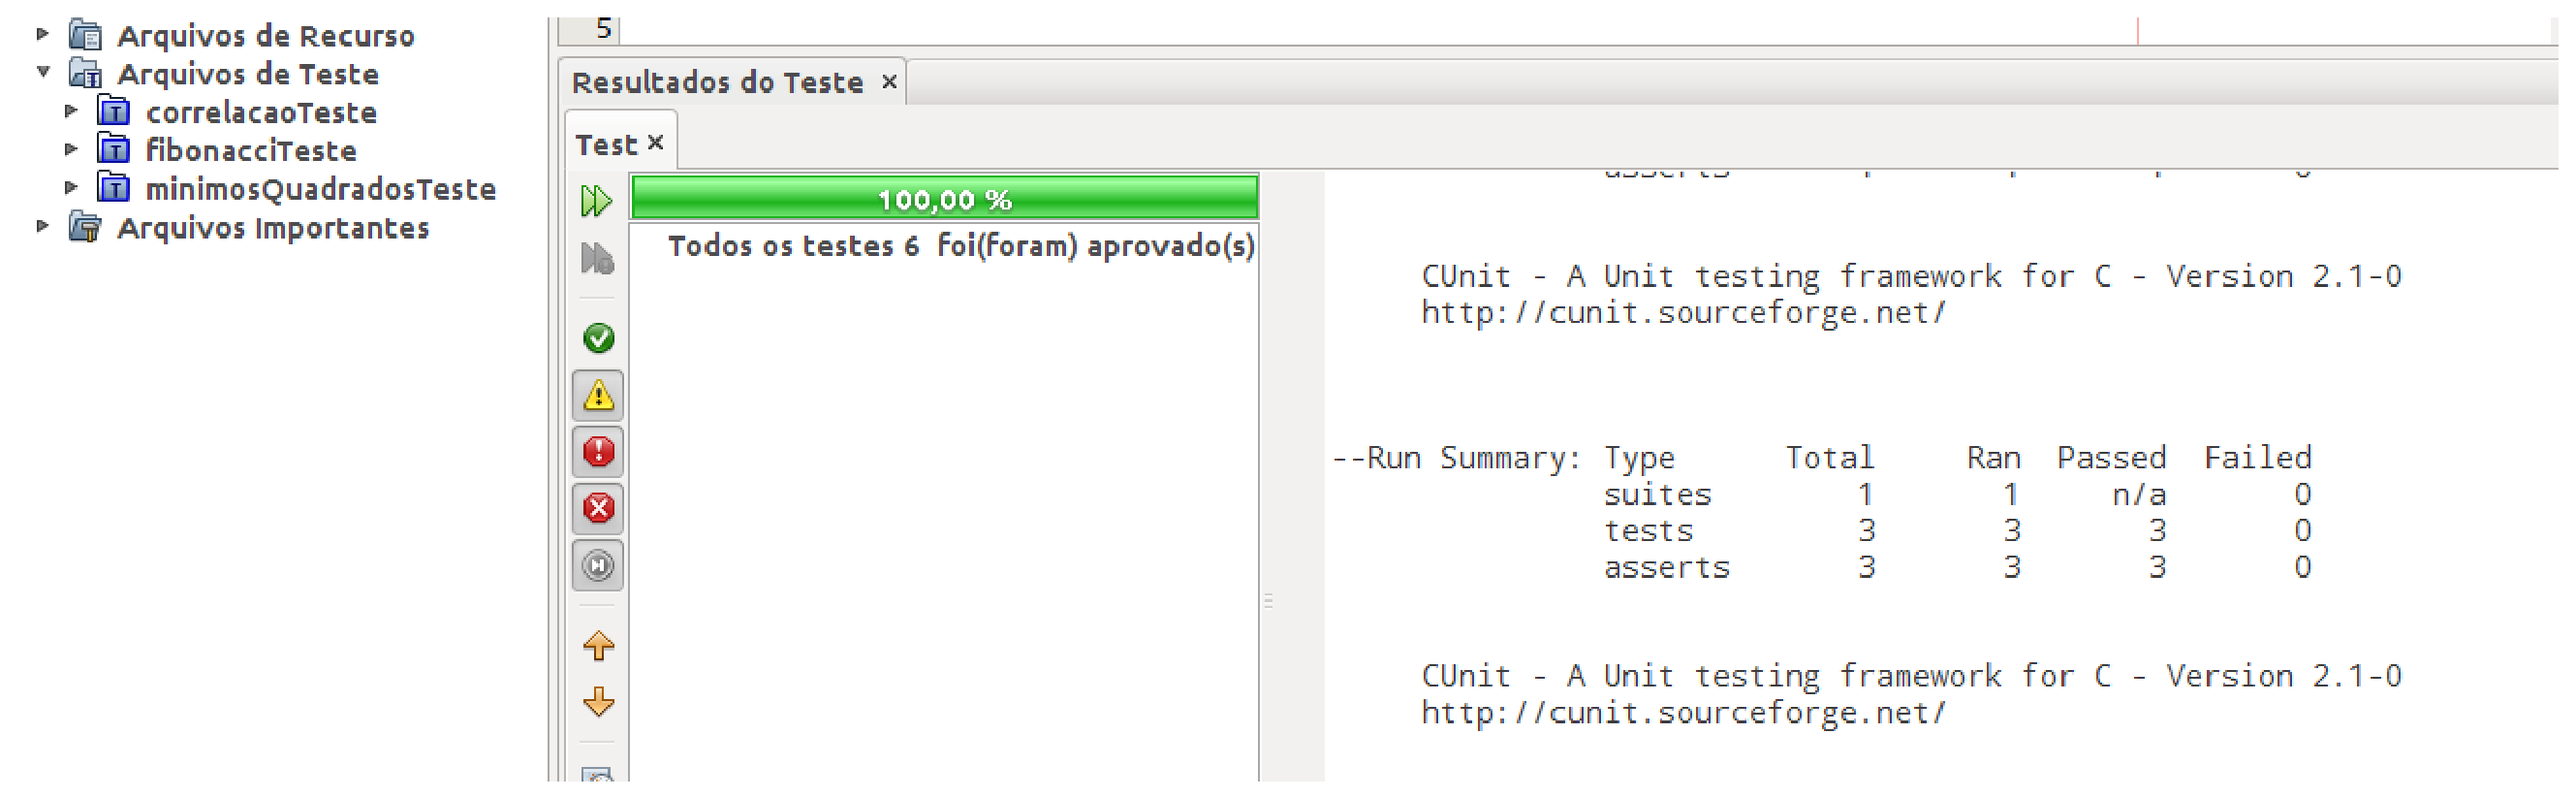
\includegraphics[width=0.9\textwidth]{figuras/coberturaEstruturado}
\caption{Cobertura de código fonte Componente Estruturado}
\label{coberturaEstrturado}
\end{figure}

A figura \ref{qualidadeEstruturado} revela o resultado da qualidade de código fonte do Componente Estruturado. É possível perceber que a métrica de números de parâmetros por método/função (ANPM) ficou nível bom no pacote de Métodos Matemáticos em C. O acoplamento (ACC) do pacote Testes dos Métodos Matemáticos em C ficou em nível bom. As demais métricas ficaram em níveis excelentes. Portanto, o código fonte do Componente Estruturado da  ferramenta InvestMVC ficou uma qualidade excelente em sua maior parte.

\begin{figure}[H]
\centering
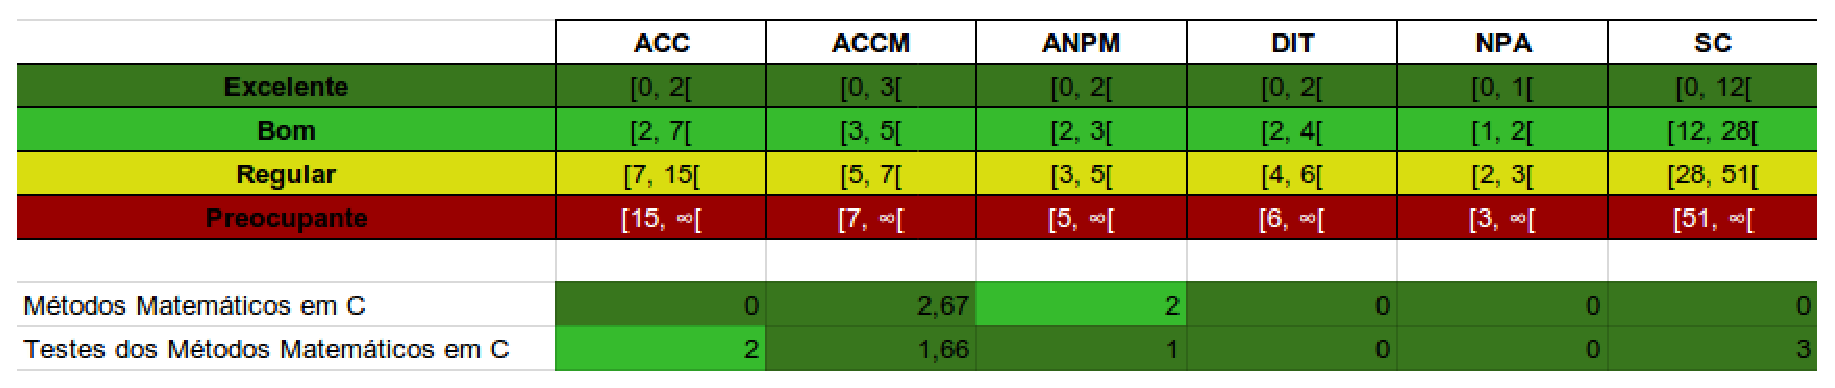
\includegraphics[width=0.9\textwidth]{figuras/qualidadeEstruturado}
\caption{Resultado da Qualidade de Código Fonte do Componente Estruturado} 
\label{qualidadeEstruturado}
\end{figure}

\section{Resultados do Componente Multiagente}

Nenhum agente do Componente Multiagente foi construído por completo. Entretanto, toda a estruturada interna desse componente já está definida conforme consta na figura \ref{estruturaSMA}.

\begin{figure}[H]
\centering
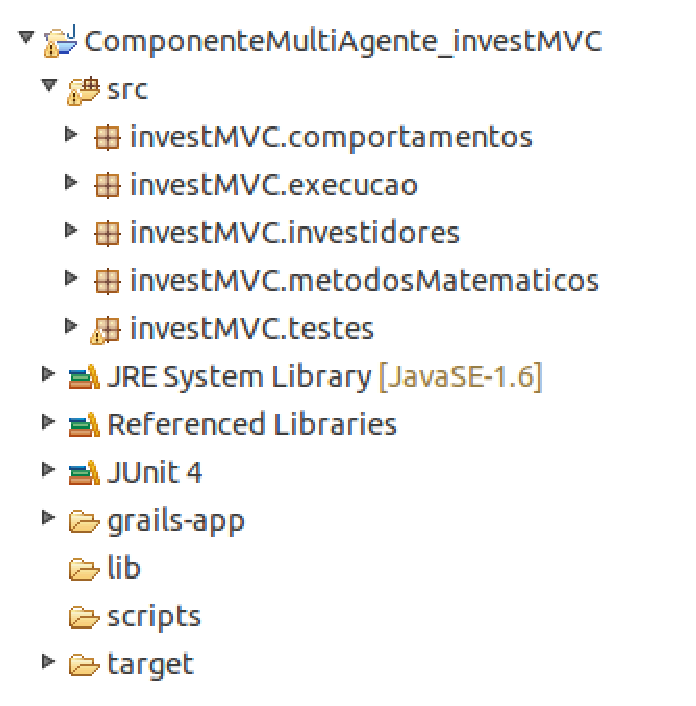
\includegraphics[width=0.5\textwidth]{figuras/estruturaSMA}
\caption{ Estrutura Interna Componente Multiagente}
\label{estruturaSMA}
\end{figure}

\section{Resultados do Componente Lógico}

Não foi feito nenhuma linha de código fonte do Componente Lógico, entretanto já foi instalada a ferramenta de teste unitário PlUnit e na mesma já foi executado um exemplo para evidenciar que a ferramenta funciona corretamente, conforme a figura \ref{prologTests}.

\begin{figure}[H]
\centering
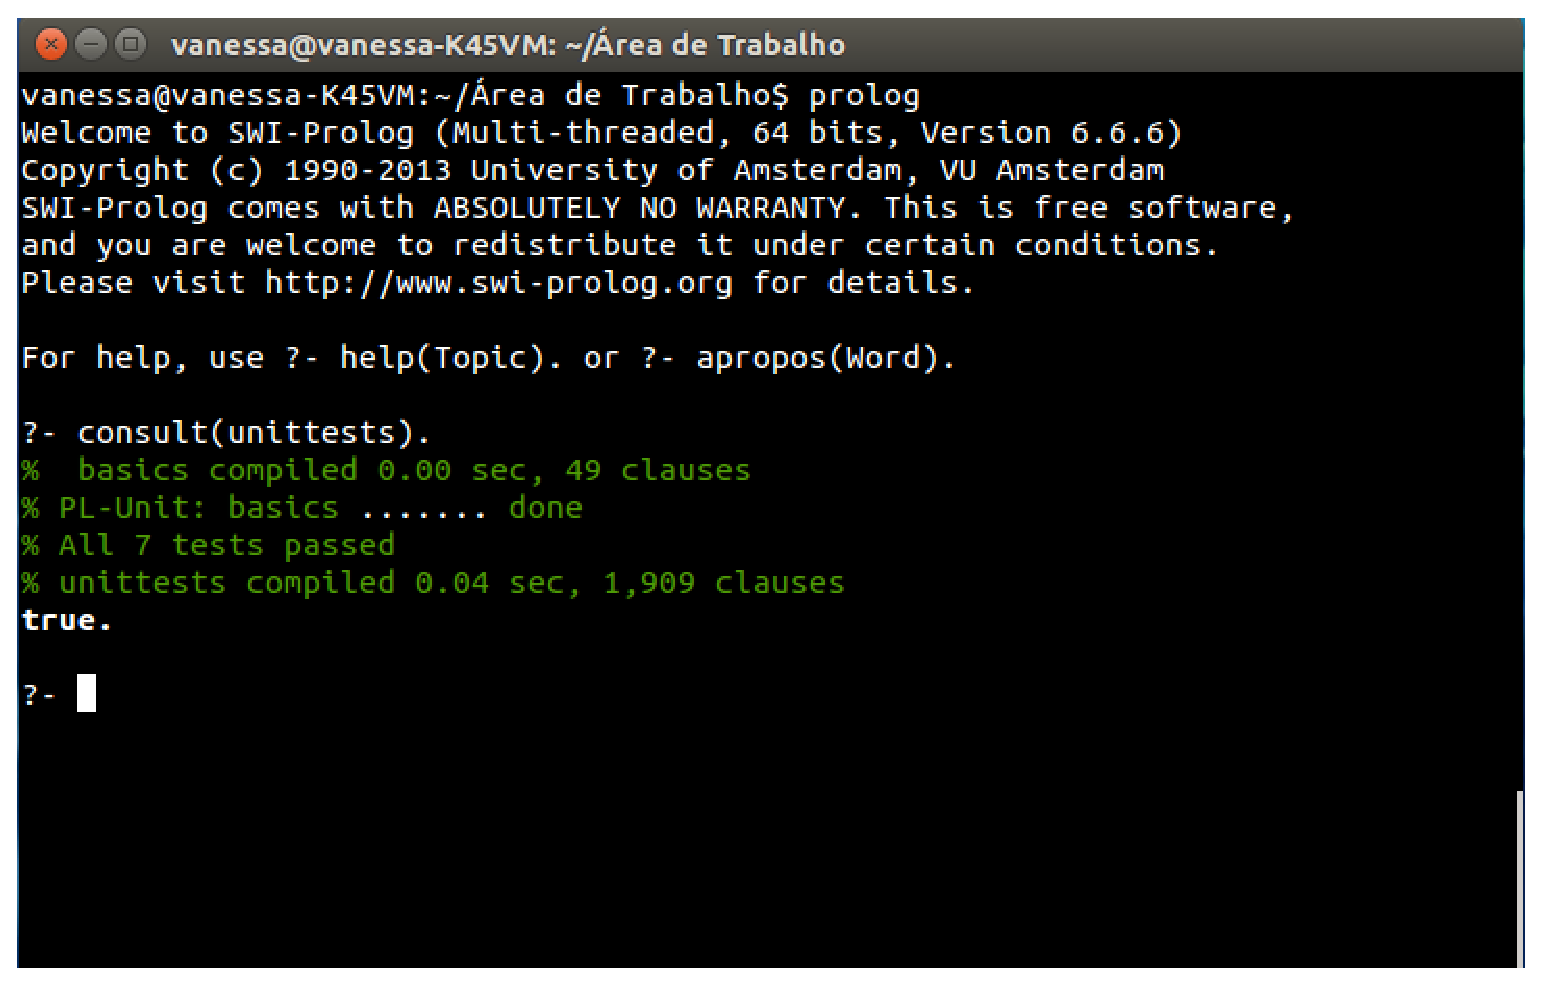
\includegraphics[width=0.9\textwidth]{figuras/prologTests}
\caption{Execução de Teste Unitário na Ferramenta PlUnit.}
\label{prologTests}
\end{figure}

\section{Resultados do Componente MQL}

No apêndice F - Componente MQL, é possível visualizar o código do Componente MQL que será responsável por interagir com a plataforma de negociação MetaTrader. É possível visualizar na figura \ref{componenteMQL}, o Componente MQL  (InvestMVC ComponenteMQL) já instalado na plataforma.

\begin{figure}[H]
\centering
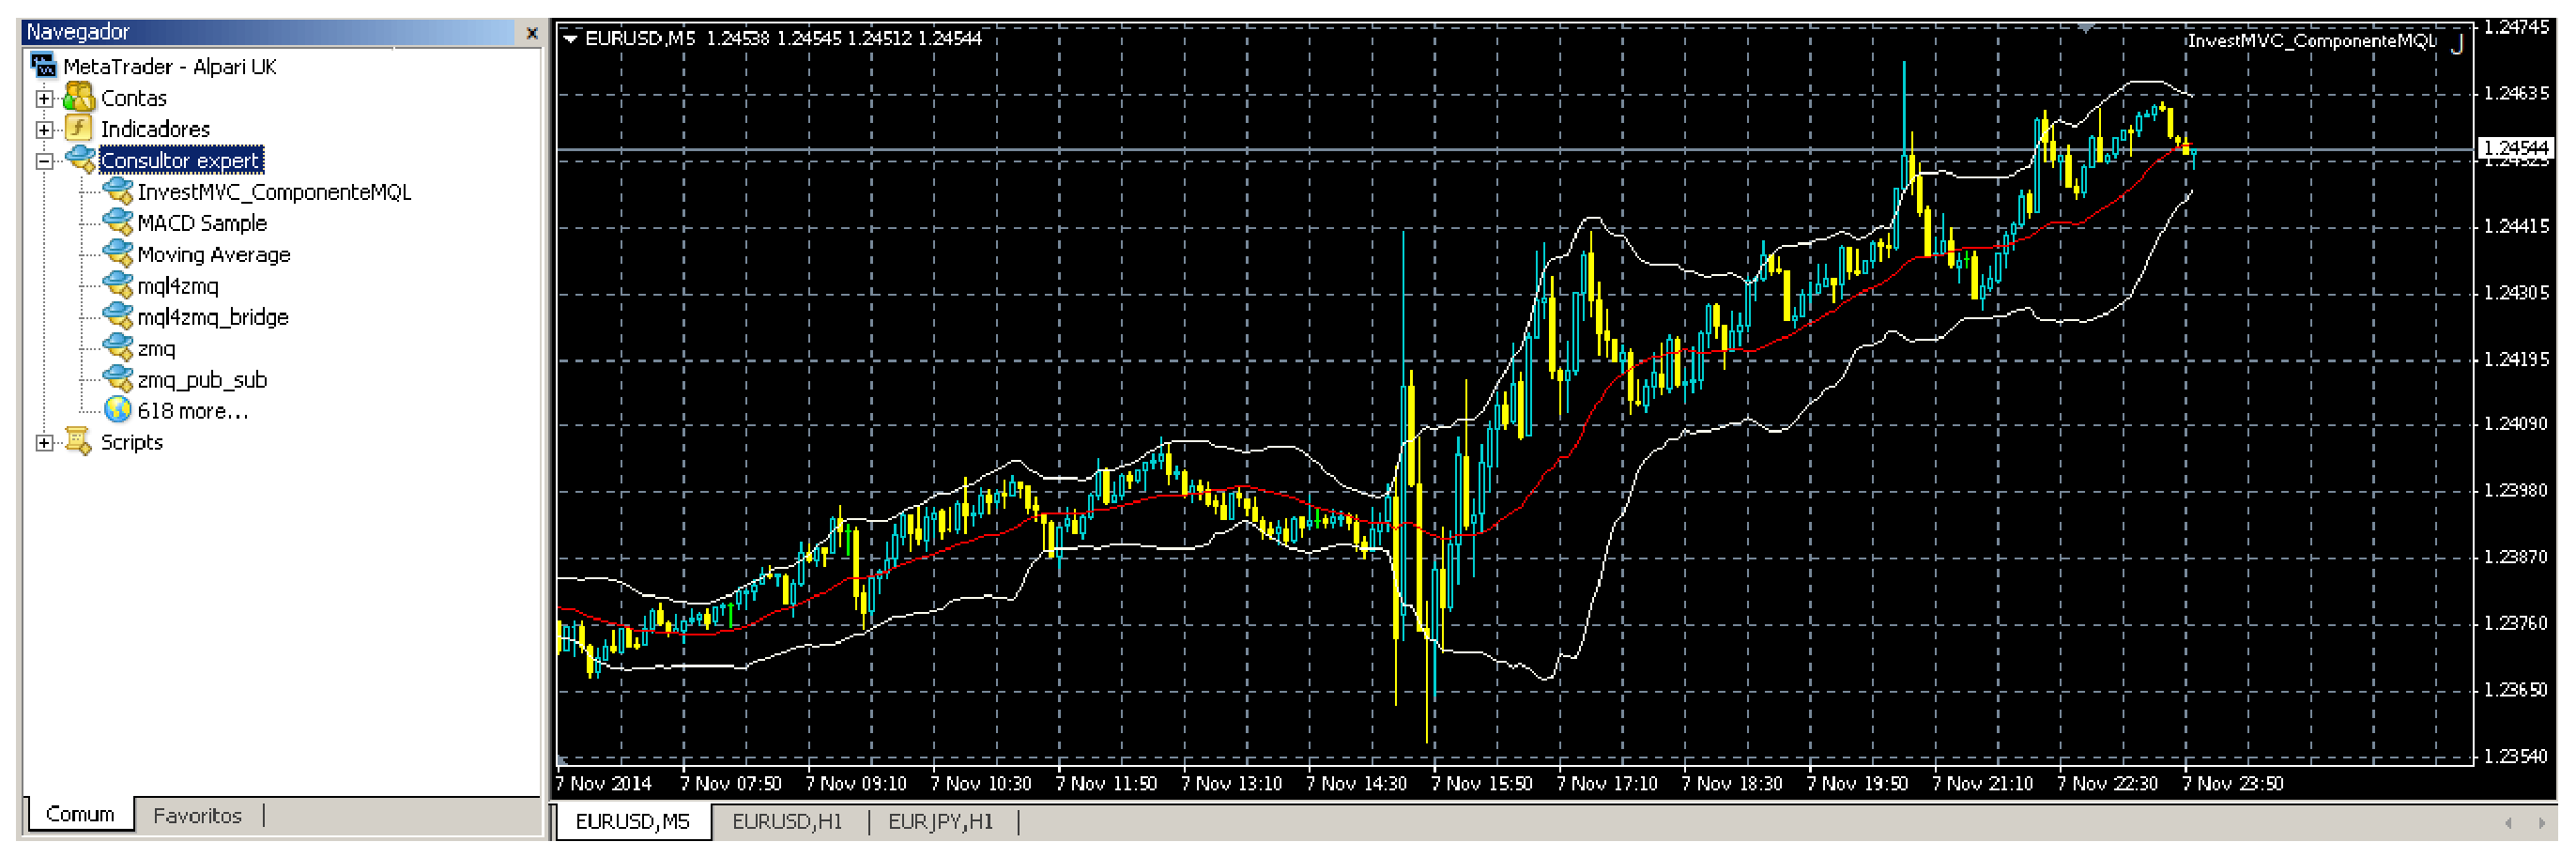
\includegraphics[width=1.0\textwidth]{figuras/componenteMQL}
\caption{Componente MQL instalado na plataforma MetaTrader}
\label{componenteMQL}
\end{figure}